\chapter{Regressões multinomial e ordinal}
\label{cap:respostas-multiplas}

A regressão logística do capítulo 7 descreve uma resposta com dois níveis. Vamos ampliar a pergunta: e se a resposta tiver três ou mais categorias? A escolha do modelo começa pelo significado dessas categorias. Uma preferência entre Texto, Vídeo e Oficina não estabelece uma ordem de qualidade. Já uma avaliação Baixa, Média e Alta possui ordem, embora a distância entre níveis não seja uma unidade de medida conhecida.

Neste capítulo, vamos ajustar modelos com apenas uma variável explicativa. Assim podemos acompanhar as contas e as probabilidades antes de acrescentar outros preditores. Os dois bancos têm 120 registros fictícios cada um; são atividades independentes, sem relação com participantes reais e sem evidência de que estudar mais cause determinada preferência ou avaliação.

\section{A pergunta orienta a escolha}

\begin{figure}[H]
\centering
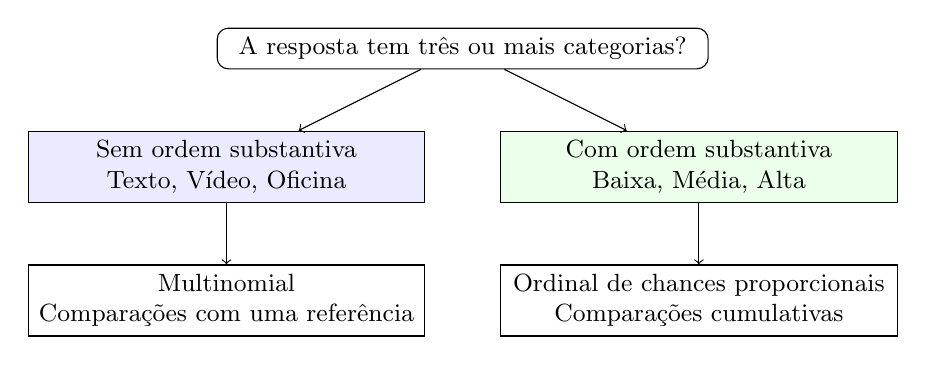
\begin{tikzpicture}[every node/.style={font=\small,align=center}]
\node[draw,rounded corners,text width=6cm] (pergunta) at (0,3.2) {A resposta tem três ou mais categorias?};
\node[draw,text width=4.8cm,fill=blue!8] (nominal) at (-3,1.7) {Sem ordem substantiva\\Texto, Vídeo, Oficina};
\node[draw,text width=4.8cm,fill=green!8] (ordinal) at (3,1.7) {Com ordem substantiva\\Baixa, Média, Alta};
\node[draw,text width=4.8cm] (m) at (-3,0) {Multinomial\\Comparações com uma referência};
\node[draw,text width=4.8cm] (o) at (3,0) {Ordinal de chances proporcionais\\Comparações cumulativas};
\draw[->] (pergunta)--(nominal); \draw[->] (pergunta)--(ordinal);
\draw[->] (nominal)--(m); \draw[->] (ordinal)--(o);
\end{tikzpicture}
\caption{Um primeiro roteiro para escolher o modelo. A ordem da resposta e os pressupostos ainda precisam ser examinados. Elaboração própria.}
\end{figure}

Não escolha regressão linear somente porque as categorias foram codificadas como 1, 2 e 3. Esses códigos podem representar rótulos. Também não transforme automaticamente uma escala ordinal em resposta binária: reunir Média e Alta, por exemplo, muda a pergunta e descarta parte da informação. Uma divisão pode ser justificável quando há uma decisão substantiva definida previamente, mas precisa ser explicada.

\section{Modelo multinomial: duas comparações, três probabilidades}

Abra \texttt{exemplo\_multinomial.csv}. Defina \texttt{id} como ID, \texttt{horas\_preparo} como contínua e \texttt{recurso} como nominal. Existem 39 escolhas de Texto, 36 de Video e 45 de Oficina. O arquivo escreve \texttt{Video} sem acento; usaremos Vídeo na narrativa. Cada linha é uma pessoa fictícia independente, e cada pessoa aparece em uma única categoria. Não informe \texttt{id} como peso nem como preditor.

Vamos adotar Texto como referência. Para $x$ horas de preparo, definimos:
\[
\eta_V(x)=a_V+b_Vx=\log\left(\frac{p_V(x)}{p_T(x)}\right),
\qquad
\eta_O(x)=a_O+b_Ox=\log\left(\frac{p_O(x)}{p_T(x)}\right).
\]
Aqui, $p_T$, $p_V$ e $p_O$ são as probabilidades das três categorias. A referência não precisa de uma terceira equação livre: as probabilidades somam 1. Portanto,
\[
D(x)=1+e^{\eta_V(x)}+e^{\eta_O(x)},\qquad
p_T(x)=\frac{1}{D(x)},\quad
p_V(x)=\frac{e^{\eta_V(x)}}{D(x)},\quad
p_O(x)=\frac{e^{\eta_O(x)}}{D(x)}.
\]
Essa transformação garante probabilidades positivas que somam 1. Não podemos ajustar duas regressões binárias isoladas e esperar que suas previsões formem automaticamente essa distribuição conjunta.

No jamovi, abra \textbf{Regressão (Regression) $\rightarrow$ Regressão Logística (Logistic Regression) $\rightarrow$ N resultados (N Outcomes, Multinomial)}. Os nomes podem variar com o idioma. Coloque \texttt{recurso} na resposta e \texttt{horas\_preparo} em covariáveis; escolha Texto como referência. Solicite coeficientes, intervalos de confiança e razões exponenciadas. A documentação oficial apresenta essas opções e a configuração das referências \parencite{JamoviMultinomial}.

Os coeficientes aproximados para este banco são:
\begin{center}
\begin{tabular}{lrrr}
\hline
Comparação & Intercepto & Horas & $e^{b}$ \\
\hline
Vídeo / Texto & $-0{,}98275$ & $0{,}34668$ & $1{,}414$ \\
Oficina / Texto & $-2{,}14541$ & $0{,}76648$ & $2{,}152$ \\
\hline
\end{tabular}
\end{center}

Para uma hora adicional, a razão $p_V/p_T$ é multiplicada por aproximadamente $1{,}414$. Isso não equivale a multiplicar a probabilidade de Vídeo por esse número. O denominador é Texto, e não a soma de todas as outras categorias. A razão de probabilidades entre duas categorias também pode ser expressa como chances condicionais de uma em relação à outra; por isso, a saída usa a expressão \textit{odds ratio}. Sempre nomeie o numerador e o denominador.

Em três horas, obtemos aproximadamente $p_T=0{,}310$, $p_V=0{,}328$ e $p_O=0{,}362$. A categoria mais provável é Oficina, mas sua probabilidade está longe de 100\%. Uma previsão de categoria não elimina a incerteza da distribuição.

\begin{figure}[H]
\centering
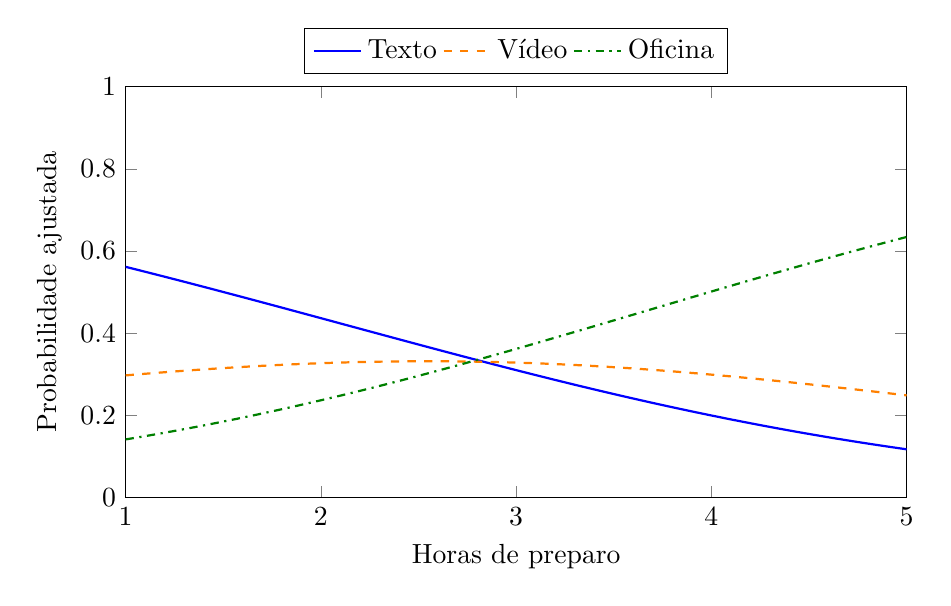
\begin{tikzpicture}
\begin{axis}[width=11.5cm,height=6.8cm,xmin=1,xmax=5,ymin=0,ymax=1,
 xlabel={Horas de preparo},ylabel={Probabilidade ajustada},xtick={1,2,3,4,5},
 legend style={at={(0.5,1.03)},anchor=south,legend columns=3},samples=100,domain=1:5]
\addplot[blue,thick] {1/(1+exp(-0.98274825+0.34668051*x)+exp(-2.14540596+0.76647838*x))};
\addlegendentry{Texto}
\addplot[orange,thick,dashed] {exp(-0.98274825+0.34668051*x)/(1+exp(-0.98274825+0.34668051*x)+exp(-2.14540596+0.76647838*x))};
\addlegendentry{Vídeo}
\addplot[green!50!black,thick,dashdotted] {exp(-2.14540596+0.76647838*x)/(1+exp(-0.98274825+0.34668051*x)+exp(-2.14540596+0.76647838*x))};
\addlegendentry{Oficina}
\end{axis}
\end{tikzpicture}
\caption{Probabilidades multinomiais calculadas com os coeficientes do exemplo. As curvas são a interpolação do modelo no intervalo observado. Elaboração própria.}
\label{fig:multinomial-probabilidades}
\end{figure}

Repare na curva de Vídeo: ela primeiro sobe e depois cai, embora $b_V$ seja positivo. A razão Vídeo/Texto aumenta em todo o intervalo, mas a probabilidade absoluta de Oficina cresce e participa do mesmo denominador. Esse exemplo mostra por que vale apresentar probabilidades junto com os coeficientes.

Trocar a referência modifica as comparações, os sinais e os coeficientes, mas não as probabilidades ajustadas para o mesmo modelo. Para comparar Oficina com Vídeo, subtraímos os dois logits: a inclinação é $0{,}76648-0{,}34668=0{,}41980$. A razão Oficina/Vídeo é multiplicada por $e^{0{,}41980}\approx1{,}522$ a cada hora.

\section{Modelo ordinal: preservando a ordem}

Agora abra \texttt{exemplo\_ordinal.csv}. São outros 120 registros fictícios. A variável \texttt{avaliacao} contém Baixa, Media e Alta, com totais 37, 42 e 41. Defina-a como ordinal e organize explicitamente os níveis na ordem \textbf{Baixa, Media, Alta}. A ordem alfabética não é a ordem substantiva. \texttt{horas\_preparo} continua sendo contínua.

O modelo de chances proporcionais reúne a informação por limites cumulativos. Há duas divisões: Baixa versus Média/Alta e Baixa/Média versus Alta. Usaremos a convenção:
\[
\log\left(\frac{P(Y\leq j\mid x)}{P(Y>j\mid x)}\right)=\theta_j-\beta x,
\qquad j=1,2;\quad \theta_1<\theta_2.
\]
O sinal negativo diante de $\beta x$ é parte da convenção. Com ela, um $\beta$ positivo favorece categorias superiores. Outros programas podem escrever a equação com sinal oposto; compare a definição antes de comparar sinais \parencite{RPolr}.

\begin{figure}[H]
\centering
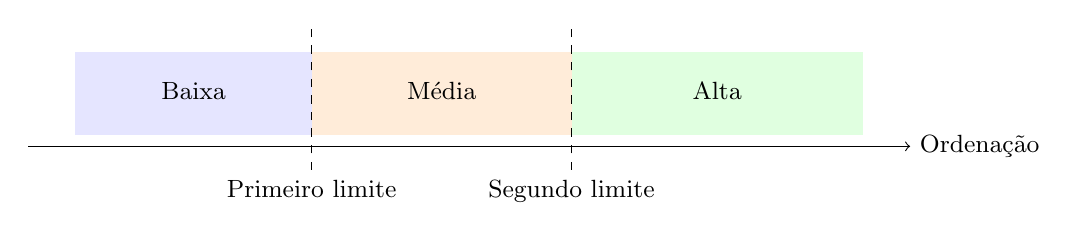
\begin{tikzpicture}[every node/.style={font=\small,align=center}]
\draw[->] (-0.6,0)--(10.6,0) node[right] {Ordenação};
\fill[blue!10] (0,0.15) rectangle (3,1.2);
\fill[orange!15] (3,0.15) rectangle (6.3,1.2);
\fill[green!12] (6.3,0.15) rectangle (10,1.2);
\node at (1.5,0.7) {Baixa}; \node at (4.65,0.7) {Média}; \node at (8.15,0.7) {Alta};
\draw[dashed] (3,-0.3)--(3,1.5); \draw[dashed] (6.3,-0.3)--(6.3,1.5);
\node[below] at (3,-0.3) {Primeiro limite};
\node[below] at (6.3,-0.3) {Segundo limite};
\end{tikzpicture}
\caption{As categorias mantêm uma ordem. A largura dos blocos é esquemática: não representa distância conhecida entre respostas nem frequência de pessoas. Elaboração própria.}
\end{figure}

Vamos transformar a equação em probabilidades. Seja $L(t)=1/(1+e^{-t})$, a função logística. Defina $F_1(x)=L(\theta_1-\beta x)$ e $F_2(x)=L(\theta_2-\beta x)$. Então:
\[
p_{\mathrm{Baixa}}=F_1,\qquad
p_{\mathrm{M\acute{e}dia}}=F_2-F_1,\qquad
p_{\mathrm{Alta}}=1-F_2.
\]
Os limiares ordenados garantem $F_2>F_1$. Observe a diferença entre categoria e acumulação: $F_2$ é a probabilidade de Baixa \textbf{ou} Média, não a probabilidade de Média sozinha.

No menu de regressão logística, selecione \textbf{Resultados ordinais (Ordinal Outcomes)}. Use \texttt{avaliacao} como resposta e \texttt{horas\_preparo} como covariável. Solicite a tabela de limiares, os coeficientes, as razões exponenciadas e os intervalos. Confira a ordem dos níveis no banco e na saída; a análise oficial disponibiliza a apresentação dos limiares \parencite{JamoviOrdinal}.

Neste exemplo, $\hat\beta=0{,}63782$, $\hat\theta_1=0{,}96293$ e $\hat\theta_2=2{,}70115$. Como a equação foi escrita para a probabilidade cumulativa inferior, $e^{\hat\beta}\approx1{,}892$ multiplica as \textbf{chances cumulativas superiores}, $P(Y>j)/P(Y\leq j)$, a cada hora. O multiplicador é o mesmo nos dois limites: esse é o pressuposto de chances proporcionais. Não significa que as probabilidades das três categorias cresçam na mesma proporção.

Em três horas, as probabilidades ajustadas são aproximadamente $0{,}279$, $0{,}409$ e $0{,}313$. Pequenas diferenças na última casa decorrem do arredondamento. Os limiares estão na escala do preditor linear; não são pontos de corte de 0,5 para classificação, nem notas mínimas observadas na escala original.

\begin{figure}[H]
\centering
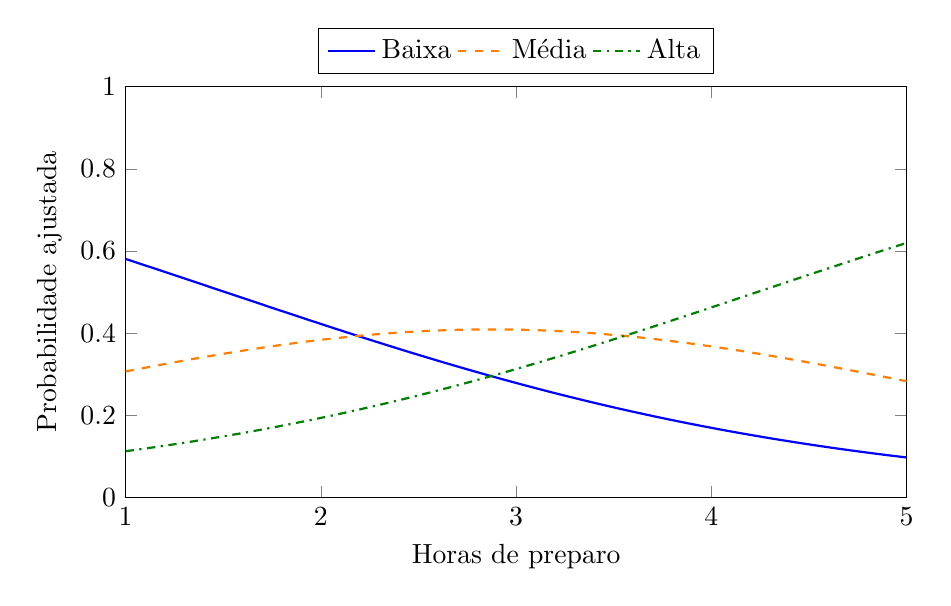
\begin{tikzpicture}
\begin{axis}[width=11.5cm,height=6.8cm,xmin=1,xmax=5,ymin=0,ymax=1,
 xlabel={Horas de preparo},ylabel={Probabilidade ajustada},xtick={1,2,3,4,5},
 legend style={at={(0.5,1.03)},anchor=south,legend columns=3},samples=100,domain=1:5]
\addplot[blue,thick] {1/(1+exp(-(0.96292747-0.63782252*x)))};
\addlegendentry{Baixa}
\addplot[orange,thick,dashed] {1/(1+exp(-(2.70115221-0.63782252*x)))-1/(1+exp(-(0.96292747-0.63782252*x)))};
\addlegendentry{Média}
\addplot[green!50!black,thick,dashdotted] {1-1/(1+exp(-(2.70115221-0.63782252*x)))};
\addlegendentry{Alta}
\end{axis}
\end{tikzpicture}
\caption{Probabilidades ordinais calculadas com um coeficiente comum e dois limiares. Elaboração própria.}
\label{fig:ordinal-probabilidades}
\end{figure}

\section{Conferindo o ajuste e reconhecendo limites}

Os dois modelos assumem observações independentes neste uso. Respostas repetidas da mesma pessoa, alunos da mesma turma ou amostras com pesos e conglomerados podem exigir outros modelos. Também precisamos examinar categorias raras, combinações vazias e relações não lineares com preditores contínuos. Não acrescente muitos termos a uma amostra pequena somente porque o software aceita a fórmula.

No modelo multinomial, uma categoria perfeitamente separada pelas variáveis pode produzir coeficientes muito grandes e dificuldades de convergência. Confira avisos, estimativas e erros padrão; mudar o número de casas decimais não resolve o problema. O ajuste também depende da escala dos preditores, como observa a documentação de \texttt{multinom} \parencite{RMultinom}.

No ordinal, o coeficiente comum é uma restrição substantiva. Podemos começar explorando as distribuições cumulativas e as relações com os preditores, mas um gráfico ou dois ajustes binários separados não comprovam o pressuposto. Se ele for inadequado, precisamos de avaliação específica e de um modelo que permita relaxá-lo; o multinomial é uma possibilidade quando faz sentido abrir mão da ordem, não uma correção automática. Não presuma que toda versão do jamovi oferece uma caixa de seleção para esse diagnóstico.

A log-verossimilhança multinomial do exemplo é aproximadamente $-120{,}995$, com quatro parâmetros e AIC $249{,}990$. No ordinal, temos log-verossimilhança $-119{,}160$, três parâmetros e AIC $244{,}319$. \textbf{Não use esses dois AICs para escolher o melhor modelo}: eles foram calculados para respostas e bancos distintos. Comparações exigem a mesma resposta, os mesmos casos e uma base de verossimilhança comparável. Os pseudo-$R^2$ também não representam a porcentagem de variância explicada no sentido da regressão linear.

Os números deste capítulo foram calculados diretamente dos CSVs por máxima verossimilhança no script didático \texttt{scripts/calcular\_categoricos.py}. Podemos ainda reproduzir o ordinal no Rj, depois de abrir seu CSV:
\begin{verbatim}
d <- data
d$avaliacao <- ordered(d$avaliacao,
    levels = c("Baixa", "Media", "Alta"))
m <- MASS::polr(avaliacao ~ horas_preparo,
    data = d, method = "logistic", Hess = TRUE)
coef(m)
m$zeta
predict(m, newdata = data.frame(horas_preparo = 1:5),
    type = "probs")
\end{verbatim}

O exemplo usa o módulo Rj apresentado no capítulo 8. A documentação de \texttt{polr} explica a parametrização e os métodos disponíveis \parencite{RPolr}. Ao relatar intervalos, registre também como foram obtidos: aproximações de Wald e intervalos por perfil de verossimilhança não precisam coincidir. Não substitua o intervalo exibido por uma conta diferente sem identificá-la.

\section{Um relato que acompanha a pergunta}

Um relato multinomial pode começar assim: ``Em 120 registros fictícios, ajustamos a escolha do recurso em função das horas de preparo, com Texto como referência. Uma hora adicional correspondeu a um multiplicador de 2,152 na razão Oficina/Texto. Em três horas, as probabilidades ajustadas foram 0,310 para Texto, 0,328 para Vídeo e 0,362 para Oficina.'' Em uma aplicação real, acrescente os intervalos, o delineamento, as exclusões, os diagnósticos e os limites de generalização.

Para o ordinal, descreva a ordem Baixa/Média/Alta e a convenção da equação. A razão cumulativa estimada de 1,892 por hora se refere às categorias superiores em cada limite, sob chances proporcionais. Evite escrever que ``a avaliação aumenta 89,2\%''; essa frase troca uma razão de chances por uma alteração direta da resposta. Os dados aqui são fictícios e o ajuste serve para aprender a interpretar, sem conclusão causal ou validação externa.

\section{Exercícios de interpretação}
\begin{enumerate}
\item Por que os códigos 1 = Texto, 2 = Vídeo e 3 = Oficina não justificam uma regressão ordinal?
\item Use o modelo multinomial para calcular a probabilidade de Oficina em três horas. Por que ela não é simplesmente $e^{\eta_O}$?
\item O coeficiente de Vídeo/Texto é positivo. Isso obriga a probabilidade de Vídeo a crescer entre quatro e cinco horas?
\item Se Oficina passar a ser a referência, o modelo precisa produzir novas probabilidades para as mesmas pessoas? Explique.
\item No ordinal, com três horas, calcule $F_1$, $F_2$ e a probabilidade da categoria Média. Qual diferença entre $F_2$ e essa probabilidade?
\item Uma pessoa compara os AICs dos dois exemplos e escolhe o ordinal por ter o menor valor. Avalie a decisão e proponha uma comparação apropriada.
\end{enumerate}

\subsection{Respostas comentadas}
\begin{enumerate}
\item Os números são rótulos; não existe ordem substantiva entre os três recursos. A escolha começa pelo significado das categorias.
\item $\eta_O=-2{,}14541+0{,}76648\times3\approx0{,}15403$. Dividindo $e^{\eta_O}$ pelo denominador comum, obtemos aproximadamente $0{,}362$. A exponencial isolada é uma razão em relação a Texto.
\item Não. A probabilidade passa de aproximadamente $0{,}299$ para $0{,}249$, enquanto a razão Vídeo/Texto continua aumentando. A probabilidade de Oficina também participa do denominador.
\item Não, desde que sejam o mesmo modelo e os mesmos casos. Mudam a parametrização e as comparações apresentadas.
\item $F_1\approx0{,}279$ e $F_2\approx0{,}687$; a probabilidade de Média é $F_2-F_1\approx0{,}409$. $F_2$ inclui Baixa e Média.
\item Os bancos e as respostas são diferentes. Podemos, por exemplo, comparar no banco ordinal o modelo apenas com limiares ao modelo com horas, mantendo os mesmos casos; a avaliação substantiva e dos pressupostos continua necessária.
\end{enumerate}

\section{Para continuar no Balaio Científico}

Como preparação, retome o post \href{https://www.balaiocientifico.com/2024/07/como-realizar-analises-de-regressao-no.html}{Como realizar análises de regressão no jamovi} e o texto sobre \href{https://www.balaiocientifico.com/2026/10/tipos-de-variaveis-no-jamovi-nominal.html}{tipos de variáveis no jamovi}. Eles ajudam a organizar a pergunta e a configuração dos dados; as equações multinomial e ordinal foram desenvolvidas neste capítulo com as referências oficiais. Na aula \href{https://www.youtube.com/watch?v=398uFqX7NRA}{Tipos de medida no jamovi}, revise a distinção entre nominal, ordinal e contínua. Depois, abra os dois bancos e registre por que cada resposta recebeu um tipo diferente.
